% Paper for CGAT
\documentclass[10pt, conference, compsocconf]{IEEEtran}

\usepackage{float}
%\usepackage{url}
\usepackage{graphicx}
\usepackage{subfig}
\usepackage{color}

\begin{document}

\title{CGAT In The Hat}

% author names and affiliations
% use a multiple column layout for up to two different
% affiliations

\author{\IEEEauthorblockN{Eriq Augustine, Ryan Hnarkis, Aldrin Montana, Ryan Verdon, Tyler Yero}
\\
\IEEEauthorblockA{Department of Computer Science\\
Cal Poly, San Luis Obispo\\
 \textsf{\{eaugusti, rhnaraki, amontana, rverdon, tyero\}@calpoly.edu}
}
}

\maketitle

\thispagestyle{empty}
\pagestyle{empty}

\section{Introduction}\label{sec:introduction}
Gene annotation is the process of associating metadata about a gene with the
contig, a dna sequence, on which the gene resides.\cite{annotation} This metadata is necessary for conducting
genomic research projects and analysis involving the contig's genomic sequence.
Currently, there is no specialty gene annotation software. Genome browsers
all maintain lots of genomic data and are used when manually annotating genes,
but do not provide a user-friendly interface. While genome browsers
will likely never be replaced (UCSC genome browser, etc. are well
established\cite{ucscbrowser, ncbi}), it would be desirable to have a software system that better
accommodates the visual and informational needs of gene annotation.

\textit{CGAT} is a web-based gene annotation application designed with
usability, simplicity, and efficiency in mind. It is not a feature-rich and data-rich
 genome browser like the \textit{UCSC genome brower}. Nor is \textit{CGAT}
designed to be a replacement for other genome browsers in any aspect other than
gene annotation. Other gene browsers attempt to accommodate many needs of the
biology community and so offer many features, and a cluttered, chaotic
interface. Gene annotation, while not a trivial task, can be well-serviced by a
simple data model. Ideally, by focusing on a simple data model, \textit{CGAT}
is able to provide a clean, streamlined experience. \textit{CGAT} aims to
provide users with a way to view gene annotations without extra, unnecessary
information obscuring their view while also embodying a Wikipedia-like emphasis
on collaboration and openness.

This paper discusses the progress that has been made this quarter and the future work that 
still needs to be done. The rest of the paper is as follows. Section \ref{sec:motive} discusses the
motivation for creating CGAT. Section \ref{sec:choice} explains why we chose MongoDB
as our backend. Section \ref{sec:implementation} goes into the details of how
our backend and frontend are implemented currently. Section \ref{sec:ui} explains the
various features of our UI. Lastly, section \ref{sec:future} describes the future work still left to
do.

\section{Motivation}\label{sec:motive}
Dr. Anya Goodman, a professor in the biochemistry department at Cal Poly, San Luis
Obispo, offers a bioinformatics course that covers several aspects of gene
annotation. Her work is a part of the Genomics Education Partnership (GEP) at 
Washington University in St. Louis.\cite{gep} The goal of GEP is to teach undergrad students
in Biology how to annotate genes and other features in raw sequence data.
The CGAT project is spearheaded by Ryan Verdon to accommodate Dr.
Goodman's needs and ideas for ideal gene annotation software.

\section{Database Choice}\label{sec:choice}
% TODO(ryan): Put decision and considereations here.
%  Schema will go in implementation section.
%  Incoude some text about how having the documents in JSON (Mongo is actually BSON) makes it really easy to use in JSON.

\section{Implementation}\label{sec:implementation}

\subsection{Backend}

\subsubsection{Database Schema}

\subsection{Frontend}

\subsubsection{Technologies}

\subsubsection{API}

\section{UI Design}\label{sec:ui}

\section{Future Work}\label{sec:future}


\bibliographystyle{acm}
\bibliography{refs}


\onecolumn
\appendices

\section{JSON Data Models}\label{sec:data_models}
\centering
Here are diagrams depicting our JSON data model.

\begin{figure*}[h]
   \centering
   \subfloat[Contig format]{\label{fig:JSON-contig}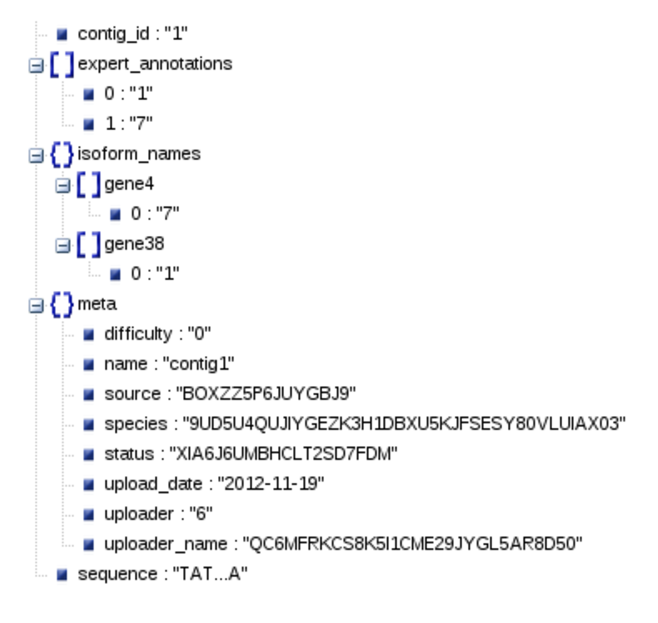
\includegraphics[height=70mm]{contig.eps}}
   \subfloat[Annotation format]{\label{fig:JSON-annotation}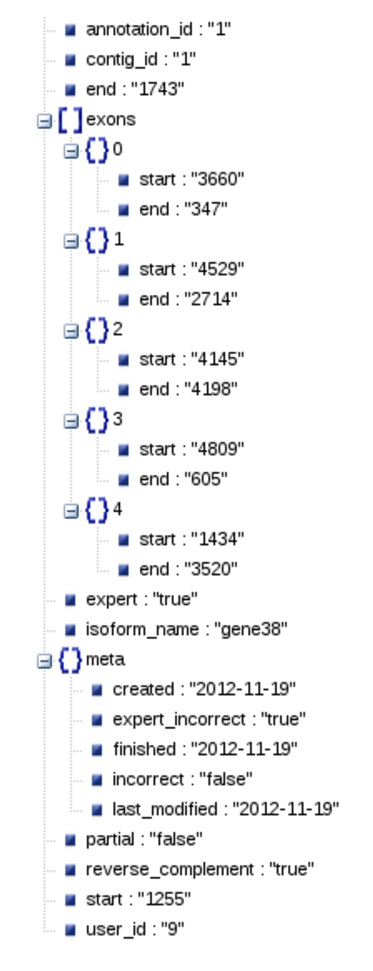
\includegraphics[height=80mm]{annotation.eps}}
   \caption{JSON format for Contigs and Annotations.}
\end{figure*}

\begin{figure*}[h]
   \centering
   \subfloat[User format]{\label{fig:JSON-user}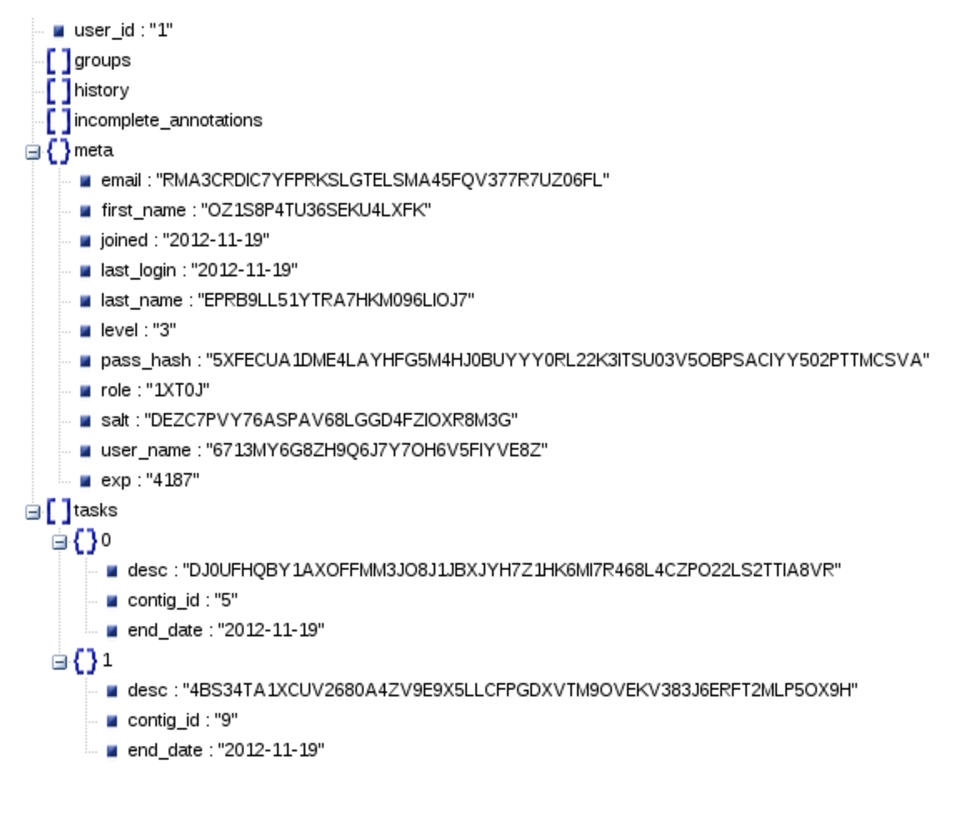
\includegraphics[height=90mm]{user.eps}}
   \subfloat[Group format]{\label{fig:JSON-group}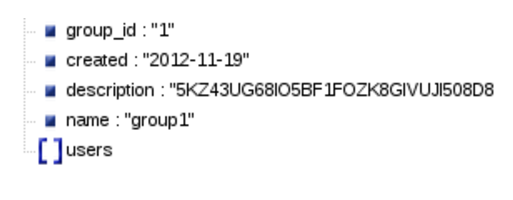
\includegraphics[height=25mm]{group.eps}}
   \caption{JSON format for Users and Groups.}
\end{figure*}


\end{document}
